\documentclass[12pt]{article}

\usepackage[margin=2cm]{geometry}
\usepackage{amsmath}
\usepackage{multicol}
\usepackage{nopageno}
\usepackage{SIunits}
\usepackage{graphicx}
\usepackage{enumerate}
\usepackage{enumitem}
%\usepackage{mathabx}
\usepackage{wasysym}

%%%%%%%%%%%%%%%%%%%%%%%%%%%%%%%%%%%%%%%%%%%%%%%%%%%%%
% For putting links in the document (both to sections and hyperlinks)
\usepackage{hyperref}
\usepackage{url}
\hypersetup{
    colorlinks=true,     % false: boxed links; true: colored links
    linkcolor=red,       % color of internal links
    citecolor=blue,      % color of links to bibliography
    filecolor=blue,      % color of file links
    urlcolor=blue        % color of external links
}
% below, use \url{http://www.nytimes.com} (they will be urlcolor)
%%%%%%%%%%%%%%%%%%%%%%%%%%%%%%%%%%%%%%%%%%%%%%%%%%%%%


%%%%%%%%%%%%%%%%%%%%%%%%%%%%%%%%%%%%%%%%%%%%%%%%%%%%%
% for the events page boxes

% boxed regions
\usepackage{tcolorbox}
\tcbuselibrary{skins,breakable}

% fonts & spacing
\usepackage{lmodern}
\usepackage{microtype}
\usepackage{calc}


% small helper macros (adjust these)
\newcommand{\boxheight}{4.2cm}   % height for each event box
\newcommand{\boxfont}{\scriptsize} % change to \tiny or \footnotesize as desired
\newcommand{\linelen}{0.95\linewidth} % timeline line length

%%%%%%%%%%%%%%%%%%%%%%%%%%%%%%%%%%%%%%%%%%%%%%%%%%%%%
\newcommand{\rmd}{\ensuremath{{\rm d}}}
%\newcommand{\vv}[1]{\ensuremath{\vec{#1}}}
\newcommand{\vv}[1]{\ensuremath{\mathbf{#1}}}
\newcommand{\ee}[1]{\ensuremath{\mathbf{e}_{#1}}}
%%%%%%%%%%%%%%%%%%%%%%%%%%%%%%%%%%%%%%%%%%%%%%%%%%%%%



\begin{document}

\begin{center}
{\Large Greenhouse Effect (Part 1): Heating by Radiation}
\end{center}

%%%%%%%%%%%%%%%%%%%%%%%%%%%%%%%%%%%%%%%%%%%%%%%%%%%%
%%%%%%%%%%                                  Questions                                %%%%%%%%%%%%%%%%
%%%%%%%%%%%%%%%%%%%%%%%%%%%%%%%%%%%%%%%%%%%%%%%%%%%%
\begin{enumerate}

\item {\bf  Calculating the temperature of the Earth (Part II)}
	%
	\begin{enumerate}
	\item We found last week in Discussion (and in Section 4.1 of your textbook) that: (i) The Sun emits a total power of about $\unit{4 \times 10^{26}}{\watt}$, where a Watt, W, is a $\frac{\text{J}}{\text{s}}$; (ii) The solar flux at the position of the Earth in orbit is about \unit{1400}{\watt/\meter^2} (this is called the ``Solar constant'', $S$); (iii) The average solar flux at the surface of the earth, ignoring albedo, is exactly $F_\text{Sun at surface (ideal avg)} = S / 4$; (iv) The albedo of the earth is about 0.3.  \underline{Review each of these four statements} with your group and then say a few words about each (what it means, how it was calculated, include a picture if it helps).
	\item Write down an equation for the average flux of the sun at the surface, $F_\text{Sun at surface, avg}$, in terms of $S$ and $\alpha$ (i.e., combining (iii) and (iv) from (a)).  Explain why it has this form and calculate a numerical value.
	\item Repeat the calculation from Q3 of Discussion last week (``Part I'') to estimate the Earth's equilibrium temperature.  Recall that we did this by assuming that $F_\text{in} = F_\text{out}$, where the incoming flux is from the sun (just found in (b)) and the outgoing flux is the Earth's blackbody radiation, $F_\text{Earth surf}$, which depends on its temperature. Discuss with your group the equilibrium temperature value you find and say a few words about it here.
	\item Let's construct an ``energy flux\footnote{This is similar to our prior ``energy flow diagram'' but now the flowing quantity is flux, energy {\em per area} per time.  As you will see in your construction, this will mean that flux is passing from one two-dimensional surface to the next (like the approximately two-dimensional atmosphere above our heads).} diagram'' associated to the calculation in part (c).  Draw a single, wide, rectangular box, representing the surface of the Earth. Draw two flux arrows, one coming into the Earth surface box from above, and one going out of the Earth surface box (also above). Although we had more precise names for these fluxes above, let's now call them $F_\text{sun}$ and $F_\text{earth}$ (label your arrows). Since we have assumed a situation of equilibrium, the Earth's total energy is constant, so you can indicate that with a horizontal arrow ($\leftrightarrow$) inside the box. Also write a $T_\text{Earth}$ inside the box to represent this constant energy value, the equilibrium temperature. We know the value for the incoming arrow; write it next to the arrow. Describe how this picture represents the equation in part (c).  What must be the value for the outgoing arrow?
	\item We will now attempt to correct the value found in (c).  Let's start by adding second ``object'' to our energy flux diagram: the atmosphere. 
		%
		\begin{itemize}
		\item Draw two wide rectangles, one above the other, with some separation. Label the bottom ``Earth's Surface'' and the top ``Atmosphere.''  
		\item The incoming flux arrow to the Earth surface that you drew in (d) remains.  Why does it go into the surface box, not\footnote{This arrow, from the sun to the Earth could go ``behind'' the atmosphere box, or around it, but should still come from the top of the page.} the atmosphere box?
		\item The outgoing flux arrow from the Earth surface also remains, but it's value might be different in the end.  This arrow does not go out into space as before. Why not?
		\item The atmosphere should have two flux arrows coming out, each will have the same value, call it $F_\text{atm}$. Why does each have the same value?
		\item Put ``unchanging'' arrows ($\leftrightarrow$) inside the boxes. Give a temperature to each box.  
		\item Which flux arrow do we know the number for? Indicate it.
		\end{itemize}
		%
	\item Let's get some equations from your flux diagram.  Use the basic principle of $F_\text{in} = F_\text{out}$ for a box, to get two equations that relate  $F_\text{sun}$, $F_\text{earth}$, and $F_\text{atm}$ (two boxes means two equations).  Get a third equation by combining the two equations to eliminate one variable.
	\item Use your equations, and the Stefan-Boltzmann equation, to get a new temperature estimate for the Earth's surface.  Is this one correct?
	\end{enumerate}

%%%%%%%%%%%%%%%%%%%%%%%%%%%%%%%%%%%%%%%%%%%%%%%%%%
\item {\bf Measuring solar incident flux:}  In Lab this week, we measure first the heat capacity of Aluminum and then use that to measure the radiant flux of a desk lamp (or if we're lucky, the Sun) by tracking the temperature increase of an aluminum block over time.
	%
	\begin{enumerate}
	\item We find in lab that the aluminum has a specific heat capacity, $c_\text{Al}$ about 4.5 times smaller than water (\unit{0.90}{\joule / \gram / \kelvin} vs.\ \unit{4.2}{\joule / \gram / \kelvin}). Write down the defining equation of the specific heat capacity, and say in your own words what it means.  Then describe in plain language what it means that the specific heat capacity of water is 4.5 times higher than aluminum (consider, e.g., \unit{10}{\gram} of each substance subjected to the same heating).  Can you make sense of the word ``capacity'' in this context?
	\item Below is a table of data taken for a \href{http://www.atmo.arizona.edu/students/courselinks/spring13/atmo170a1s1/online_course/week_5/solar_irrad_expt.html}{class from University of Arizona} (where the Sun is a more reliable partner).  Let's try to estimate the solar constant\footnote{If you point your aluminum block perpendicular to the rays of the sun, and you have a clear sky, then you should be able to estimate $S$, not the average flux including albedo and the average over the whole Earth's surface!}, $S$, using the data.\\[6pt]
		%
		\begin{minipage}[t]{0.4\textwidth}
		\vspace{0pt}
		\begin{itemize}[leftmargin=1.8em,labelsep=0.6em]
		\item Using graph paper, plot this data (Temperature (C) vs.\ time (s)) being careful to set the range on each axis so that no space is wasted (look at the minimum and maximum values of each quantity). 
		\item Exam the data and choose a range of times where the temperature seems to be increasing approximately linearly (away from the initial and final ``flatness''). 
		\end{itemize}
		\end{minipage} 
		\hfill %
		\begin{minipage}[t]{0.40\textwidth}%
		\vspace{0pt}
		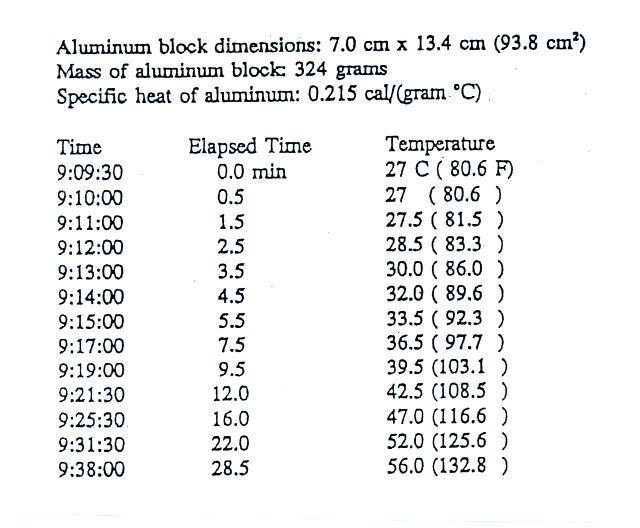
\includegraphics[width=\textwidth]{images/example-data_solar-irradiance_weidman-arizona.jpg}
		\end{minipage}\\
		%
		\begin{itemize}[leftmargin=1.8em,labelsep=0.6em]
		\item	What is the average temperature of the aluminum during that time interval?  
		\item Use a ruler to draw a line of best fit through this portion of the data (you can draw the straight line across your whole graph, but only fit to your chosen data points).
		\item Find the slope of that line and its units (always use two widely-separated points {\em on the line} to find a slope, not data points).
		\item The slope you found is $\frac{\Delta T}{\Delta t}$ for the aluminum block.  Now use the defining equation for specific heat capacity and the specific heat of aluminum (\unit{0.9}{\joule/\gram/\kelvin}) to determine the power gain of the aluminum, $\frac{\Delta E}{\Delta t}$.
		\item Draw an energy flux diagram for the aluminum block.  You should have two\footnote{You could have flux arrows out of the block into the insulating styrofoam, but those will be approximately cancelled by flux arrows into the aluminum from the styrofoam, so we need only include the arrows in/out of the sky-facing surface.} flux arrows.  In this case, the block is {\em not} in equilibrium, so you should have an arrow inside the box showing the direction of energy change.
		\item This diagram implies a non-equilibrium equation of the form:
			%
			\begin{equation*}
			\begin{split}
			\frac{\Delta E}{\Delta t} &= \frac{\Delta E_\text{in}}{\Delta t} - \frac{\Delta E_\text{out}}{\Delta t} \\
			\frac{\Delta E}{\Delta t}  & = F_\text{block} \, A_\text{block} - F_\text{sun} \,A_\text{block}
			\end{split}
			\end{equation*}
			%
		We calculated the left-hand side number from our graph. The block area, $A_\text{block}$, can be calculated from the data in the table (convert to meters).  We know the value of the flux of the block outward from its average temperature and the Stefan-Boltzmann law. The flux from the sun is our unknown variable; solve for it!
		\end{itemize}
	\end{enumerate}
	
\item {\bf Freezing water in the desert night (BONUS in F2025)}: When it is nighttime, we don't get the Sun's incoming flux.  Luckily, all of the objects around us have retained energy throughout the day, and radiate their own infrared light (heat) to keep us relatively warm until sunrise.    If, however, you can restrict an object's line of sight to only the sky --- and insulate it thermally to minimize conduction from the ground and air --- then you will find that it quickly radiates away its heat into the sky!  
	%
	\begin{enumerate}
	\item You made a number of temperature measurements of the sky using your infrared thermometer.  What was the average value you (and your classmates) found?  Recall that we have the data results in a google survey from the first weeks of class.
	\item Using the same equation as the previous question, estimate the rate of energy change, $\frac{\Delta E}{\Delta t}$, of a puddle of water.  How long would it take the water to decrease from $20\degree$C to the freezing point?
	\end{enumerate}

\end{enumerate}
	
%%%%%%%%%%%%%%%%%%%%%%%%%%%%%%%%%%%%%%%%%%%%%%%%
%%%%%%%%%%%%%      astronomical info           %%%%%%%%%%%%%%%%%%%%%
%%%%%%%%%%%%%%%%%%%%%%%%%%%%%%%%%%%%%%%%%%%%%%%%


%\newpage
%\thispagestyle{empty}
%\mbox{}

%\newpage
%%%%%%%%%%%%%%%%%%%%%%%%%%%%%%%%%%%%%%%%%%%%%%%%%%%%
%%%%%%%%%%                           Extras                           %%%%%%%%%%%%%%
%%%%%%%%%%%%%%%%%%%%%%%%%%%%%%%%%%%%%%%%%%%%%%%%%%%%




%%%%%%%%%%%%%%%%%%%%%%%%%%%%%%%%%%%%%%%%%%%%%%%%%%%%
%%%%%%%%%%                                  References                                %%%%%%%%%%%%%%%%
%%%%%%%%%%%%%%%%%%%%%%%%%%%%%%%%%%%%%%%%%%%%%%%%%%%%
%\noindent {\bf Data Sources}: 



\end{document}
